% !TeX program = pdflatex
\documentclass[tikz,border=8pt]{standalone}
\usepackage{tikz}\usetikzlibrary{calc}
\definecolor{FigureBlue}{HTML}{2563EB}\definecolor{FigureOrange}{HTML}{EA580C}
\begin{document}
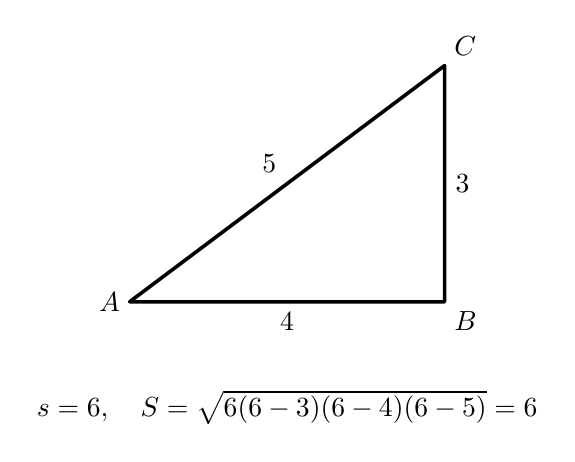
\begin{tikzpicture}[line cap=round,line join=round]
  \coordinate (A) at (0,0); \coordinate (B) at (4,0); \coordinate (C) at (4,3);
  \draw[line width=1.3pt] (A)--node[below] {$4$}(B)--node[right] {$3$}(C)--node[above left] {$5$}(A);
  \node[left] at (A) {$A$}; \node[below right] at (B) {$B$}; \node[above right] at (C) {$C$};
  \node[below=10mm] at ($(A)!.5!(B)$) {$s=6,\quad S=\sqrt{6(6-3)(6-4)(6-5)}=6$};
\end{tikzpicture}
\end{document}
